\documentclass[journal]{./IEEE/IEEEtran}
\usepackage{cite,graphicx}
\usepackage{multirow}

\newcommand{\SPTITLE}{Distributing Parts of a Matrix from Master to Slaves Over Sockets with Multi-threading and CPU Affinity}
\newcommand{\ADVISEE}{Jadon C. Sacayanan}
% \newcommand{\ADVISER}{Adviser M. Name}

\newcommand{\BSCS}{Bachelor of Science in Computer Science}
\newcommand{\ICS}{Institute of Computer Science}
\newcommand{\UPLB}{University of the Philippines Los Ba\~{n}os}
\newcommand{\REMARK}{\thanks{Presented to the Faculty of the \ICS, \UPLB\
                             in partial fulfillment of the requirements
                             for the Degree of \BSCS}}
        
\markboth{CMSC 180 Introduction to Parallel Computing, \ICS}{}
\title{\SPTITLE}
% \author{\ADVISEE~and~\ADVISER%
\author{\ADVISEE
\REMARK
}
\pubid{\copyright~2025~ICS \UPLB}

%%%%%%%%%%%%%%%%%%%%%%%%%%%%%%%%%%%%%%%%%%%%%%%%%%%%%%%%%%%%%%%%%%%%%%%%%%

\begin{document}

% TITLE
\maketitle

% ABSTRACT
\begin{abstract}
    This research examines the performance of a multi-threaded master-slave architecture for distributing parts of a matrix using sockets, both within a single PC and across multiple PCs. The study compares scenarios with and without CPU affinity. The focus is on the average runtime as the number of slaves increases. Results indicate that increasing the number of slaves reduces runtime significantly, with distributed computing across multiple machines showing the best performance. 
\end{abstract}

% INDEX TERMS
\begin{keywords}
parallel computing, multi-threading, CPU affinity, Z-score normalization, matrix computation
\end{keywords}

% INTRODUCTION
\section{Introduction}
Efficient data processing is crucial in high-performance computing, where optimizing computational tasks can significantly improve execution speed. When managing large datasets, data can be distributed to enable parallel processing, which may reduce processing time and improve overall performance.

% \subsection{Z-score normalization}
% The Z-score indicates how far a value deviates from the mean, measured in standard deviations, ensuring that all measurements are on the same scale\cite{andrade2021z}.
% All distributions expressed in Z-scores have the same mean (0) and the same variance (1). This allows Z-scores to be used in comparing observations coming from different distributions \cite{abdi2007z}.
% To compute for the Z-score, we use the formula:
% \begin{equation}
% \label{zscoreformula}
%     z=\frac{x-\mu}{\sigma}
% \end{equation}
% where:
% \( x \) is the observed value,  
% \( \mu \) is the mean, and
% \( c \) is the standard deviation.

% In columnar Z-score normalization, each column in a matrix is normalized independently by applying the Z-score formula to every value.
% For each column, the mean and standard deviation are computed separately, and each value is transformed by subtracting the column's mean and dividing by its standard deviation.
% Since Z-scores standardize measurements to the same scale by effectively removing units, they allow for the comparison of values that were originally measured in different units \cite{abdi2007z}.

\subsection{Distributed computing}
Distributed computing refers to programs that make calls to other address spaces, which may reside on the same machine or potentially on remote machines. This includes technologies such as remote object invocation, where tasks are distributed across different systems, allowing for the execution of processes on separate nodes and facilitating efficient resource utilization in a networked environment
\cite{waldo1996note}.

\subsection{Socket programming}
Socket programming is a way of connecting two nodes on a network to communicate with each other. One socket(node) listens on a particular port at an IP, while the other socket reaches out to the other to form a connection. The server forms the listener socket while the client reaches out to the server \cite{socketc}.

\subsection{Thread}
A thread is an abstract entity that represents the execution of a sequence of instructions within a program.
It is a lightweight component consisting of essential elements like registers, a stack, and other associated data.
A thread is the smallest unit of execution, capable of being scheduled and executed independently on a CPU.
Each thread can run independently, allowing multiple threads to execute in parallel, thereby improving the efficiency of the program \cite{lewis1996pthreads}.

\subsection{CPU affinity}
CPU affinity is a technique that binds a thread or process to a specific CPU core, preventing the operating system from migrating it to another core.
CPU affinity is optimizing cache performance.
When a thread is bound to a specific core, it can take advantage of the cache's contents, reducing cache misses and improving performance \cite{love2003kernel}.


\subsection{Cache awareness}
When the processor needs to access data, it first checks its cache.
If the data is found in the cache, it is called a cache hit, allowing for fast retrieval.
However, if the data is not present, a cache miss occurs, requiring the processor to fetch the data from main memory, which is significantly slower.

The processor does not work by retrieving a single byte of data, but instead fetches a larger block of memory called a cache line.
By loading an entire cache line at once, the processor increases the likelihood that future memory accesses will be served from the cache rather than requiring additional slow memory fetches.
This reduces the frequency of cache misses and enhances overall processing efficiency \cite{newhehe}.

\subsection{Temporal locality}
Programs has the tendency to repeatedly use the same data items during their execution. This principle is the basis for caching and suggests that it is beneficial to store frequently accessed instructions or data items nearby for future use \cite{jacob2010memory}.


% TODO : cite https://www.csc.tntech.edu/pdcincs/resources/modules/plugged/false_sharing/Cache%20Awareness-Cpp.pdf


% OBJECTIVES
\section{Objectives}
    This research activity aims to analyze the performance and efficiency of distributing matrix computations across multiple processes using socket communication.
    Specifically, it aims to:
\begin{enumerate}
    \item Implement a master-slave architecture that distributes submatrices to multiple processes via socket communication.
    \item Investigate the impact of varying the number of slave processes (t) on the execution time of matrix distribution tasks.
    \item Compare the performance when all processes are run on a single machine versus when processes are distributed across multiple physical machines.
    \item Evaluate the effect of core-affinity on communication efficiency when processes execute on the same physical machine.
\end{enumerate}


% MATERIALS AND METHODS
\section{Materials and Methods}
A program was developed to distribute parts of an n x n matrix from a master to multiple slave machines using sockets. For each matrix size n, the distribution process was executed three times to calculate the average runtime. To ensure accurate measurements, all tests were conducted under controlled conditions with no other applications running, minimizing external influences on network and system performance.


\subsection{The program}
The program is written in C and begins by prompting the user to input three values: n, the size of the square matrix; p, the port number used for socket communication; and s, a value that determines the role of the program, where 0 indicates a master and 1 indicates a slave. These inputs define how the program will behave during the matrix distribution process.



\subsection{Master}
When the program is run as a master, it generates an n × n random square matrix. The matrix is then divided into submatrices, each with n columns and approximately n/t rows, where t is the number of slaves. If n is not exactly divisible by t, the remaining rows are distributed among the first few slaves, with each receiving at most one additional row. Rather than creating separate matrices, the master identifies the start and end row indices for each submatrix, referencing the original matrix directly.

Once all submatrices are determined, the master establishes socket connections to the slave machines. It then sends each submatrix, number by number, to its assigned slave. After transmission, the master waits for an acknowledgment from each slave to confirm that the submatrix was received successfully.

\subsection{Slave}
When the program is run as a slave, it waits for a connection from the master. Upon connection, the slave receives the submatrix data, transmitted number by number, and stores it in a dynamically allocated array sized according to the expected number of rows and columns. After successfully receiving the entire submatrix, the slave sends an acknowledgment back to the master to confirm receipt. Once the communication is complete, the socket connection is closed.

\subsection{Threading}
The program uses the pthread library to create threads. In both the master and slave roles, each thread is responsible for handling a single socket connection, starting from establishing the connection (sending or listening) until the communication is closed. This design allows concurrent handling of multiple connections, enabling parallel distribution and reception of submatrices.

\subsection{CPU affinity}
The program determines the number of available cores using the sysconf function and assigns each thread to a specific core using the CPU affinity feature. To ensure system stability and prevent resource contention, one core is reserved for main system processes, such as the operating system scheduler, background services, and essential system tasks. Each thread is pinned to a dedicated CPU core using the CPU set function, preventing the operating system from migrating threads between cores and reducing interference from other system functions. This avoids the overhead of thread migration and maximizes program performance.

% \subsection{Computing for the columnar Z-score normalization}
% To compute the z-score normalization of a two-dimensional matrix, a loop traverses across the columns of the matrix.

% In each column, a loop computes the mean by taking the sum of all elements in the column and dividing the result by the height of the column.
% The standard deviation is also computed using a loop by taking the square root of the sum of the squared differences between each element and the mean, divided by the height of the column.

% Finally, the z-score for each element is calculated using Formula \ref{zscoreformula} and directly stored in the same array.
% No temporary matrices are created since the original matrix is modified in place with the help of pointers.

% These computations are done by each individual thread on the submatrix assigned to it.


\subsection{Time measurement}
The program uses the sys/time.h header to measure execution time by capturing a timestamp with gettimeofday() immediately before establishing a connection. A second timestamp is recorded after the socket is closed. The elapsed time is then calculated by determining the difference between these two timestamps. This time measurement only includes the communication phase and does not account for the preparation of the threads, such as setting up their arguments.


\subsection{Distributed computing}
The program utilizes four machines, running up to four instances of the slave program on each machine. Different configurations were used depending on the value of n. For n=2, two machines were used, each running one instance of the slave. For n=4, four machines were used with one instance of the slave on each. For n=8, the same four machines were used, each running two instances of the slave. Finally, for n=16, all four machines ran four instances of the slave each.

It also utilized a personlaized one-to-many broadcast mechanism, where the master node efficiently sends data to multiple slave nodes simultaneously. This approach minimizes communication overhead by leveraging non-blocking socket operations, ensuring that the master can continue transmitting data to other nodes without waiting for acknowledgments from previously contacted nodes.



% \subsection{Program Setup}
% By default, the program accesses the matrix in a column-major order. An additional setup was implemented to process the matrix in a row-major order.


\subsection{System information}
The program was executed on an Acer desktop equipped with an Intel® Core™ i7-8700 processor (3.20 GHz) and 16GB of memory, running Ubuntu 22.04.5 LTS. Both the master and all slave machines used the same hardware and software configuration.

% RESULTS AND DISCUSSION
\section{Results and Discussion}
The program was executed independently for three iterations for each setup, recording the runtime or elapsed time for each execution.

% Please add the following required packages to your document preamble:
% \usepackage{multirow}
% Please add the following required packages to your document preamble:
% \usepackage{multirow}

\subsection{Distributed computing with slaves running on different machines}

\begin{table}[]
\begin{center}
    \caption{Runtime Executions for Different n and t values in seconds for Distributed Computing on Different Machines}
    \begin{tabular}{|c|c|ccc|c|}
    \hline
    \multirow{2}{*}{\textbf{n}} & \multirow{2}{*}{\textbf{t}} & \multicolumn{3}{c|}{\textbf{Time Elapsed (seconds)}} & \multirow{2}{*}{\textbf{\begin{tabular}[c]{@{}c@{}}Average\\ Runtime\end{tabular}}} \\ \cline{3-5}
     &  & \multicolumn{1}{c|}{\textbf{Run 1}} & \multicolumn{1}{c|}{\textbf{Run 2}} & \textbf{Run 3} &  \\ \hline
    20000 & 2 & \multicolumn{1}{c|}{158.073970} & \multicolumn{1}{c|}{161.382508} & 154.220397 & 157.892292 \\ \hline
    20000 & 4 & \multicolumn{1}{c|}{92.240668} & \multicolumn{1}{c|}{88.906241} & 94.108334 & 91.751748 \\ \hline
    20000 & 8 & \multicolumn{1}{c|}{66.350505} & \multicolumn{1}{c|}{68.771319} & 64.112398 & 66.411407 \\ \hline
    20000 & 16 & \multicolumn{1}{c|}{49.856434} & \multicolumn{1}{c|}{50.602118} & 47.981374 & 49.479975 \\ \hline
    25000 & 2 & \multicolumn{1}{c|}{258.821180} & \multicolumn{1}{c|}{267.093215} & 252.543018 & 259.485804 \\ \hline
    25000 & 4 & \multicolumn{1}{c|}{143.290254} & \multicolumn{1}{c|}{140.113850} & 146.001709 & 143.135271 \\ \hline
    25000 & 8 & \multicolumn{1}{c|}{110.955387} & \multicolumn{1}{c|}{108.144267} & 113.589460 & 110.896371 \\ \hline
    25000 & 16 & \multicolumn{1}{c|}{72.869340} & \multicolumn{1}{c|}{74.302138} & 70.004250 & 72.391909 \\ \hline
    30000 & 2 & \multicolumn{1}{c|}{371.310715} & \multicolumn{1}{c|}{377.498020} & 365.918605 & 371.575780 \\ \hline
    30000 & 4 & \multicolumn{1}{c|}{179.321567} & \multicolumn{1}{c|}{183.927205} & 175.203491 & 179.484088 \\ \hline
    30000 & 8 & \multicolumn{1}{c|}{161.082212} & \multicolumn{1}{c|}{164.189404} & 158.440373 & 161.237330 \\ \hline
    30000 & 16 & \multicolumn{1}{c|}{138.598874} & \multicolumn{1}{c|}{136.221670} & 141.785209 & 138.868584 \\ \hline
    \end{tabular}
    \label{multi}
\end{center}
\end{table}

\begin{figure}
    \centering
    \fbox{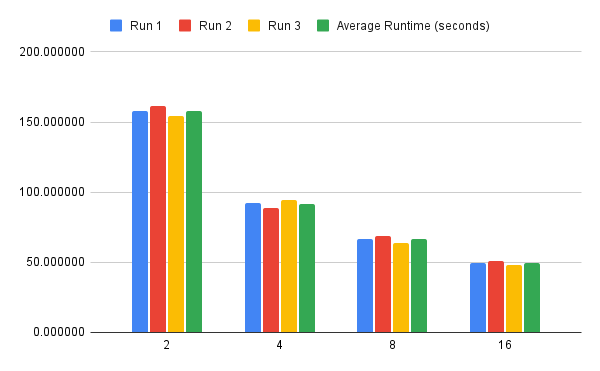
\includegraphics[width=0.45\textwidth]{images/multi_chart}}
    \caption{Runtime Executions for n=20000 in seconds for Distributed Computing on Different Slaves using Different Machines}
    \label{multi_chart}
\end{figure}

Table \ref{multi} shows the average runtime for distributing an n x n matrix using t threads across different slaves running on different machines. The results indicate that as the number of slaves increases, the runtime decreases significantly.

For a square matrix of size 20,000, the slowest runtime of approximately 157.89 seconds is observed when using 2 slaves. In contrast, the fastest runtime of approximately 49.48 seconds is achieved when using 16 slaves. This trend is visualized in Figure \ref{multi_chart}, where the runtime consistently decreases as the number of slaves increases.

\subsection{Distributed computing with slaves running on a single machine without core affinity}

\begin{table}[]
\begin{center}
    \caption{Runtime Executions for Different n and t values in seconds for Distributed Computing on Different Slaves using a Single Machine without Core Affinity}
    \begin{tabular}{|c|c|ccc|c|}
    \hline
    \multirow{2}{*}{\textbf{n}} & \multirow{2}{*}{\textbf{t}} & \multicolumn{3}{c|}{\textbf{Time Elapsed (seconds)}} & \multirow{2}{*}{\textbf{\begin{tabular}[c]{@{}c@{}}Average\\ Runtime\end{tabular}}} \\ \cline{3-5}
     &  & \multicolumn{1}{c|}{\textbf{Run 1}} & \multicolumn{1}{c|}{\textbf{Run 2}} & \textbf{Run 3} &  \\ \hline
    20000 & 2 & \multicolumn{1}{c|}{164.150009} & \multicolumn{1}{c|}{166.822194} & 160.485729 & 163.819311 \\ \hline
    20000 & 4 & \multicolumn{1}{c|}{106.496193} & \multicolumn{1}{c|}{109.841512} & 104.219304 & 106.852336 \\ \hline
    20000 & 8 & \multicolumn{1}{c|}{111.433945} & \multicolumn{1}{c|}{108.756837} & 113.275409 & 111.155397 \\ \hline
    20000 & 16 & \multicolumn{1}{c|}{209.123130} & \multicolumn{1}{c|}{202.578341} & 211.892084 & 207.864518 \\ \hline
    25000 & 2 & \multicolumn{1}{c|}{257.352387} & \multicolumn{1}{c|}{263.091982} & 254.305673 & 258.250014 \\ \hline
    25000 & 4 & \multicolumn{1}{c|}{174.123655} & \multicolumn{1}{c|}{176.452399} & 171.009812 & 173.861955 \\ \hline
    25000 & 8 & \multicolumn{1}{c|}{169.091237} & \multicolumn{1}{c|}{173.208420} & 165.877304 & 169.392320 \\ \hline
    25000 & 16 & \multicolumn{1}{c|}{344.907369} & \multicolumn{1}{c|}{337.122408} & 352.610193 & 344.879990 \\ \hline
    30000 & 2 & \multicolumn{1}{c|}{369.370952} & \multicolumn{1}{c|}{362.041733} & 375.008091 & 368.806925 \\ \hline
    30000 & 4 & \multicolumn{1}{c|}{254.110043} & \multicolumn{1}{c|}{260.344552} & 247.812063 & 254.088886 \\ \hline
    30000 & 8 & \multicolumn{1}{c|}{247.671020} & \multicolumn{1}{c|}{251.493800} & 241.520991 & 246.895270 \\ \hline
    30000 & 16 & \multicolumn{1}{c|}{512.400644} & \multicolumn{1}{c|}{523.108477} & 505.287190 & 513.598770 \\ \hline
    \end{tabular}
    \label{nca}
\end{center}
\end{table}

\begin{figure}
    \centering
    \fbox{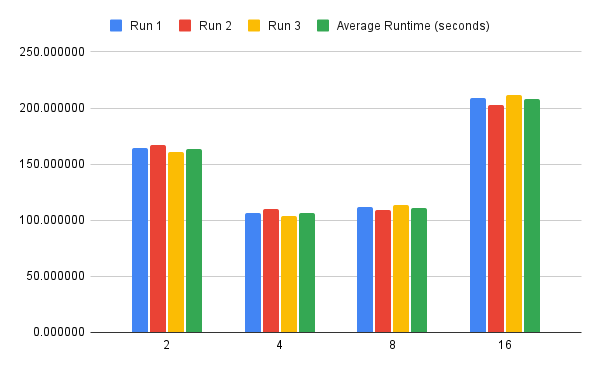
\includegraphics[width=0.45\textwidth]{images/nca_chart}}
    \caption{Runtime Executions for n=20000 in seconds for Distributed Computing on Different Slaves using a Single Machine without Core Affinity}
    \label{nca_chart}
\end{figure}

Table \ref{nca} shows the average runtime for distributing an n x n matrix using t threads across different slaves running on a single machine without core affinity. The results indicate that as the number of threads increases, the runtime initially decreases but then starts to increase again after t=8.

For a square matrix of size 20,000, the fastest runtime of approximately 106.85 seconds is observed when using 4 threads. However, when the number of threads is increased to 16, the runtime increases significantly to approximately 207.86 seconds. This trend is visualized in Figure \ref{nca_chart}, where the runtime decreases initially but rises sharply as the number of threads exceeds the number of physical cores.

\subsection{Distributed computing with slaves running on a single machine with core affinity}

\begin{table}[]
\begin{center}
    \caption{Runtime Executions for Different n and t values in seconds for Distributed Computing on Different Slaves using a Single Machine with Core Affinity}
    \begin{tabular}{|c|c|ccc|c|}
    \hline
    \multirow{2}{*}{\textbf{n}} & \multirow{2}{*}{\textbf{t}} & \multicolumn{3}{c|}{\textbf{Time Elapsed (seconds)}} & \multirow{2}{*}{\textbf{\begin{tabular}[c]{@{}c@{}}Average\\ Runtime\end{tabular}}} \\ \cline{3-5}
     &  & \multicolumn{1}{c|}{\textbf{Run 1}} & \multicolumn{1}{c|}{\textbf{Run 2}} & \textbf{Run 3} &  \\ \hline
    20000 & 2 & \multicolumn{1}{c|}{165.097044} & \multicolumn{1}{c|}{168.201223} & 162.89451 & 165.3975923 \\ \hline
    20000 & 4 & \multicolumn{1}{c|}{160.935094} & \multicolumn{1}{c|}{159.723} & 161.889234 & 160.8491093 \\ \hline
    20000 & 8 & \multicolumn{1}{c|}{101.691484} & \multicolumn{1}{c|}{104.229843} & 99.875621 & 101.932316 \\ \hline
    20000 & 16 & \multicolumn{1}{c|}{46.703392} & \multicolumn{1}{c|}{47.115298} & 45.834002 & 46.55089733 \\ \hline
    25000 & 2 & \multicolumn{1}{c|}{268.059515} & \multicolumn{1}{c|}{270.64312} & 265.202891 & 267.9685087 \\ \hline
    25000 & 4 & \multicolumn{1}{c|}{255.063759} & \multicolumn{1}{c|}{254.829371} & 258.140574 & 256.0112347 \\ \hline
    25000 & 8 & \multicolumn{1}{c|}{159.475293} & \multicolumn{1}{c|}{162.008734} & 158.027191 & 159.8370727 \\ \hline
    25000 & 16 & \multicolumn{1}{c|}{75.655035} & \multicolumn{1}{c|}{76.308295} & 74.981402 & 75.648244 \\ \hline
    30000 & 2 & \multicolumn{1}{c|}{392.014359} & \multicolumn{1}{c|}{390.202773} & 395.451002 & 392.5560447 \\ \hline
    30000 & 4 & \multicolumn{1}{c|}{342.224166} & \multicolumn{1}{c|}{345.11498} & 341.338267 & 342.892471 \\ \hline
    30000 & 8 & \multicolumn{1}{c|}{232.154717} & \multicolumn{1}{c|}{229.119456} & 234.203887 & 231.82602 \\ \hline
    30000 & 16 & \multicolumn{1}{c|}{98.284437} & \multicolumn{1}{c|}{99.087141} & 97.652309 & 98.34129567 \\ \hline
    \end{tabular}
    \label{ca}
\end{center}
\end{table}

\begin{figure}
    \centering
    \fbox{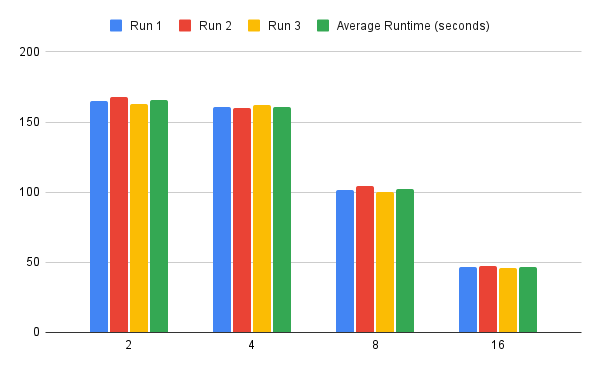
\includegraphics[width=0.45\textwidth]{images/ca_chart}}
    \caption{Runtime Executions for n=20000 in seconds for Distributed Computing on Different Slaves using a Single Machine with Core Affinity}
    \label{ca_chart}
\end{figure}

Table \ref{ca} shows the average runtime for distributing an n x n matrix using t threads across different slaves running on a single machine with core affinity. The results indicate that as the number of threads increases, the runtime decreases significantly, even for higher thread counts.

For a square matrix of size 20,000, the fastest runtime of approximately 46.55 seconds is observed when using 16 threads. This trend is visualized in Figure \ref{ca_chart}, where the runtime consistently decreases as the number of threads increases.


% CONCLUSION AND FUTURE WORK
\section{Conclusion and Future Work}
Parallel computing enhances program performance by distributing workloads across multiple nodes, enabling efficient utilization of computational resources. The results validate that increasing the number of nodes generally reduces runtime, as observed in both distributed and single-machine setups.

For distributed computing across multiple machines, increasing the number of slaves significantly improved performance, with runtimes decreasing as the number of slaves increased. This highlights the benefits of leveraging distributed systems for large-scale computations.

On a single machine, the use of core affinity showed mixed results. While core affinity aims to optimize cache utilization and reduce thread migration overhead, the implementation without core affinity was faster in some cases. This suggests that the system's scheduling algorithm may already optimize thread placement effectively, and the manual implementation of core affinity might introduce additional overhead. When the number of threads exceeds the number of available cores, the implementation without core affinity experiences a significant increase in runtime.

In conclusion, optimizing performance in parallel computing requires an approach that considers hardware capabilities, memory access patterns, and system-level optimizations. This study provides a foundation for further exploration of efficient parallel and distributed computing techniques.

% % APPENDICES
% \appendices

% \section{Proof of the First Zonklar Equation}
% Appendix one text goes here...

% \section{}
% Appendix two (without title) text goes here...

% % ACKNOWLEDGMENT
% \section*{Acknowledgment}
% Many thanks to...

% BIBLIOGRAPHY
\bibliographystyle{./IEEE/IEEEtran}
\bibliography{./cs190-ieee}
% \nocite{*}

% % BIOGRAPHY
% \begin{biography}[{
\includegraphics{./yourPicture.eps}}]{Student M. Name}
% Biography text here...
% \end{biography}


\end{document}
 
